\documentclass[aspectratio=169,11pt]{beamer}
\usetheme{Madrid}
\usecolortheme{default}
\usepackage{lmodern}
\usepackage{microtype}
\usepackage{graphicx}
\usepackage{tikz}
\usetikzlibrary{arrows.meta}
\usepackage{xcolor}

\definecolor{APBlue}{HTML}{17395C}
\definecolor{APBlueDark}{HTML}{102B45}
\definecolor{APTeal}{HTML}{168C87}
\definecolor{APOrange}{HTML}{C96B32}
\definecolor{Ink}{HTML}{1E2F40}
\definecolor{Muted}{HTML}{5E7185}
\definecolor{PaleBlue}{HTML}{EEF4F9}
\graphicspath{{../../Visual-Plan/assets/exports/figures/}{../../Visual-Plan/assets/diagrams/}}

\setbeamercolor{structure}{fg=APBlue}
\setbeamercolor{palette primary}{fg=white,bg=APBlue}
\setbeamercolor{palette secondary}{fg=white,bg=APBlueDark}
\setbeamercolor{palette tertiary}{fg=white,bg=APBlue}
\setbeamercolor{palette quaternary}{fg=white,bg=APBlueDark}
\setbeamercolor{frametitle}{fg=white,bg=APBlue}
\setbeamercolor{title}{fg=white}
\setbeamercolor{subtitle}{fg=white}
\setbeamercolor{normal text}{fg=Ink,bg=white}
\setbeamercolor{block title}{fg=white,bg=APBlue}
\setbeamercolor{block body}{fg=Ink,bg=PaleBlue}
\setbeamercolor{alerted text}{fg=APOrange}
\setbeamercolor{example text}{fg=APTeal}
\setbeamercolor{author in head/foot}{fg=white,bg=APBlueDark}
\setbeamercolor{title in head/foot}{fg=white,bg=APBlue}
\setbeamercolor{date in head/foot}{fg=white,bg=APBlueDark}
\setbeamerfont{title}{family=\rmfamily,series=\bfseries,size=\fontsize{17}{21}\selectfont}
\setbeamerfont{subtitle}{family=\sffamily,size=\fontsize{12}{15}\selectfont}
\setbeamerfont{frametitle}{family=\rmfamily,series=\bfseries,size=\fontsize{14}{17}\selectfont}
\setbeamerfont{normal text}{family=\rmfamily,size=\fontsize{15}{19}\selectfont}
\setbeamerfont{block title}{family=\rmfamily,series=\bfseries,size=\fontsize{14}{17}\selectfont}
\setbeamerfont{block body}{family=\rmfamily,size=\fontsize{15}{19}\selectfont}
\setbeamertemplate{navigation symbols}{}
\setbeamertemplate{itemize item}{\color{APBlue}$\blacktriangleright$}
\setbeamertemplate{blocks}[rounded][shadow=false]
\setbeamertemplate{frametitle continuation}{}
\setbeamersize{text margin left=0.72cm,text margin right=0.72cm}
\setlength{\leftmargini}{1.35em}

\title[Scarcity and Resource Allocation]{Scarcity and Resource Allocation}
\subtitle{AP Microeconomics · Unit 1 · Session 01}
\author[AP Microeconomics]{AP Microeconomics}
\institute[Unit 1]{Unit 1 · Session 01}
\date{}
\newcommand{\blue}[1]{\textcolor{APBlue}{\textbf{#1}}}
\newcommand{\teal}[1]{\textcolor{APTeal}{\textbf{#1}}}
\newcommand{\orange}[1]{\textcolor{APOrange}{\textbf{#1}}}
\newcommand{\muted}[1]{\textcolor{Muted}{#1}}
\newcommand{\prompt}[1]{\begin{center}\Large\color{APBlue}\textit{#1}\end{center}}
\newcommand{\answerline}{\rule{0.78\linewidth}{0.5pt}}

\begin{document}

\begin{frame}[plain]\titlepage\end{frame}

% Opening: question -> lesson target
\begin{frame}<1-2>{A fixed resource forces a choice}
  \only<1>{\vfill\prompt{A town has a fixed amount of land, labor, and time.}\vspace{0.18cm}\begin{center}\Large It chooses to produce more school meals.\end{center}\vfill\begin{center}\muted{What must happen to another use?}\end{center}}
  \only<2>{\vspace{0.25cm}\begin{block}{Today we will answer}\Large How does scarcity create a choice, a trade-off, and an opportunity cost?\end{block}\vspace{0.25cm}\begin{itemize}\setlength{\itemsep}{0.20cm}\item identify the scarce resource;\item explain the allocation decision;\item name the best alternative given up.\end{itemize}}
\end{frame}

\begin{frame}{Official targets for Session 01}
  \begin{block}{By the end of the lesson}\large I can connect a limited resource to a specific choice and a specific foregone alternative.\end{block}
  \vspace{0.25cm}\begin{itemize}\setlength{\itemsep}{0.20cm}\item Define resources and explain why \blue{scarcity creates trade-offs}.\item Answer \blue{what, how, and for whom}.\item Compare \blue{market, command, and mixed systems}.\item Explain \orange{opportunity cost} as the best alternative given up.\end{itemize}
  \vfill\begin{center}\small\muted{College Board CED: MKT-1.A · MKT-1.B}\end{center}
\end{frame}

% Scarcity: resource visual -> constraints -> conclusion
\begin{frame}<1-3>{Scarcity turns resources into trade-offs}
  \begin{columns}[T,totalwidth=\textwidth]
    \column{0.58\textwidth}\centering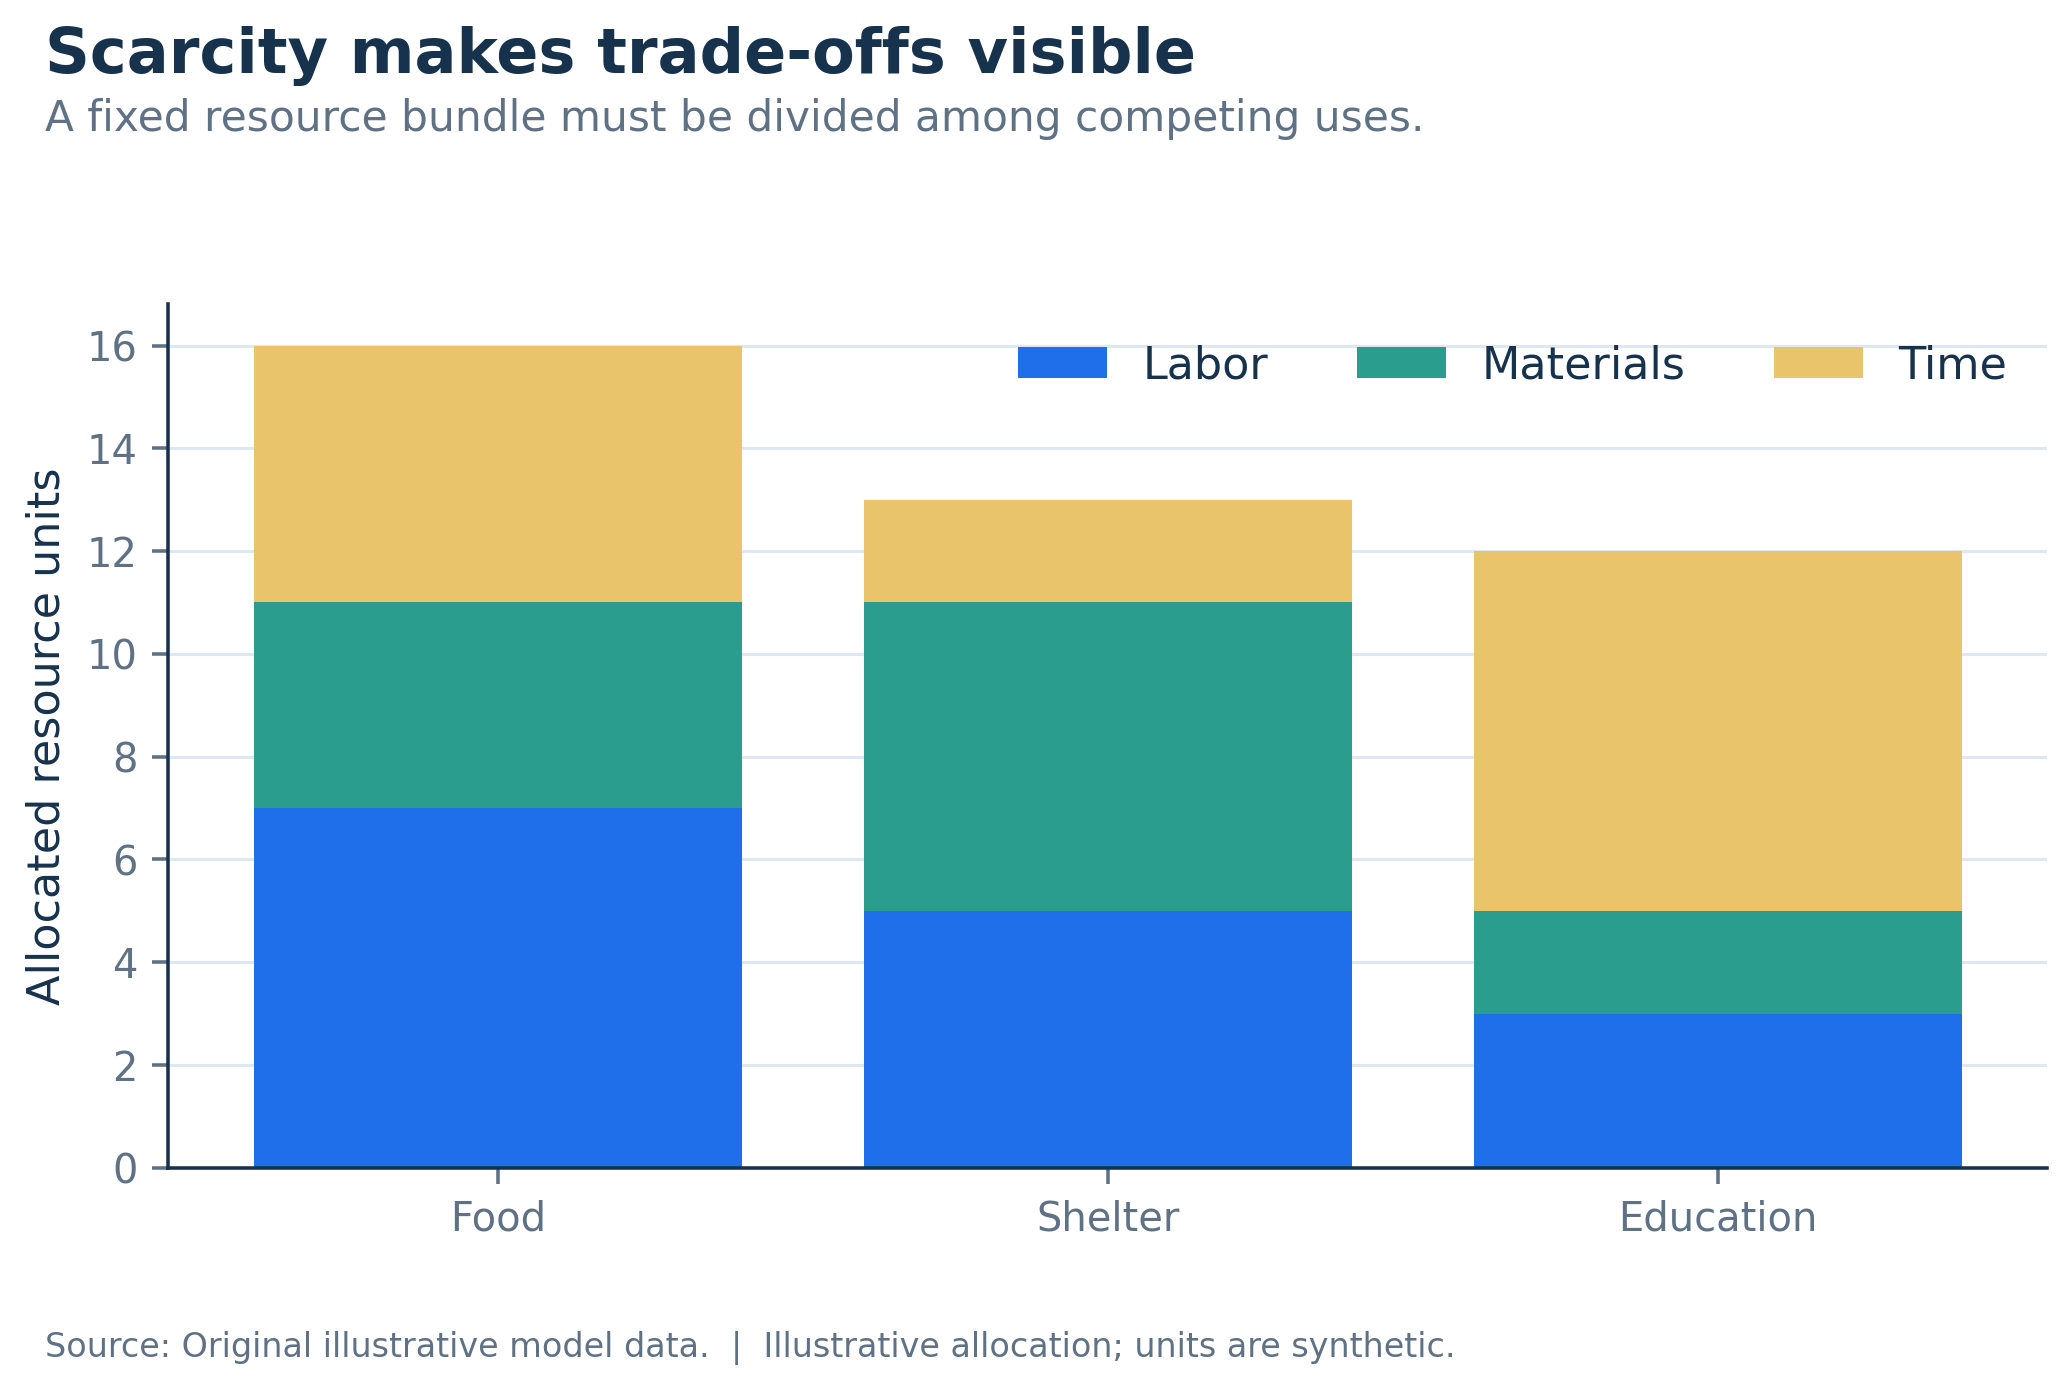
\includegraphics[width=0.92\linewidth,height=0.56\textheight,keepaspectratio]{session-01-three-resource-scarcity-panel.png}
    \column{0.36\textwidth}
      \only<1>{\vspace{0.8cm}\Large\blue{Look first.}\par\vspace{0.18cm}What resources appear limited?}
      \only<2>{\vspace{0.25cm}\Large\blue{Three constraints}\par\vspace{0.15cm}\begin{itemize}\setlength{\itemsep}{0.16cm}\item labor\item materials\item time\end{itemize}\vspace{0.12cm}Each input has competing uses.}
      \only<3>{\vspace{0.25cm}\Large\blue{Conclusion}\par\vspace{0.15cm}Desired uses exceed available resources.\vspace{0.18cm}Every decision creates an \orange{economic trade-off}.}
  \end{columns}
\end{frame}

% Definitions: definition -> mechanism -> conclusion
\begin{frame}<1-3>{The causal chain}
  \vfill\begin{center}
    \only<1>{\Huge\blue{Scarcity}\par\vspace{0.25cm}\Large Resources are limited relative to desired uses.}
    \only<2>{\Huge\blue{Choice}\par\vspace{0.25cm}\Large A decision-maker selects one use for a scarce resource.}
    \only<3>{\Huge\orange{Opportunity cost}\par\vspace{0.25cm}\Large The value of the best alternative given up.}
  \end{center}\vfill
\end{frame}

% Allocation questions: what -> how -> for whom -> synthesis
\begin{frame}<1-4>{Every economic system answers three questions}
  \begin{columns}[T,totalwidth=\textwidth]
    \column{0.31\textwidth}\only<1->{\Large\blue{What?}\par\vspace{0.15cm}Which goods or services will be made?}
    \column{0.31\textwidth}\only<2->{\Large\teal{How?}\par\vspace{0.15cm}Which methods and inputs will be used?}
    \column{0.31\textwidth}\only<3->{\Large\orange{For whom?}\par\vspace{0.15cm}Who will receive the output?}
  \end{columns}
  \vfill\only<4>{\begin{block}{Why all three matter}\large Fixed staff, time, and building capacity make all three questions unavoidable.\end{block}}
\end{frame}

% Economic systems: frame -> market -> command -> mixed/conclusion
\begin{frame}<1-4>{Economic systems coordinate scarce resources}
  \only<1>{\vfill\prompt{A system is a way of coordinating choices.}\vfill}
  \only<2->{\begin{columns}[T,totalwidth=\textwidth]\column{0.31\textwidth}\only<2->{\Large\blue{Market}\par\vspace{0.15cm}Prices, incentives, and voluntary exchange guide decisions.}\column{0.31\textwidth}\only<3->{\Large\orange{Command}\par\vspace{0.15cm}Central planning and administrative direction guide decisions.}\column{0.31\textwidth}\only<4->{\Large\teal{Mixed}\par\vspace{0.15cm}Markets operate alongside public rules or provision.}\end{columns}\vfill\only<4>{\begin{center}\muted{The coordinating mechanism changes; scarcity remains.}\end{center}}}
\end{frame}

% Resource bundle: image -> labels -> trade-off
\begin{frame}<1-3>{A resource bundle can support competing uses}
  \begin{columns}[T,totalwidth=\textwidth]\column{0.60\textwidth}\centering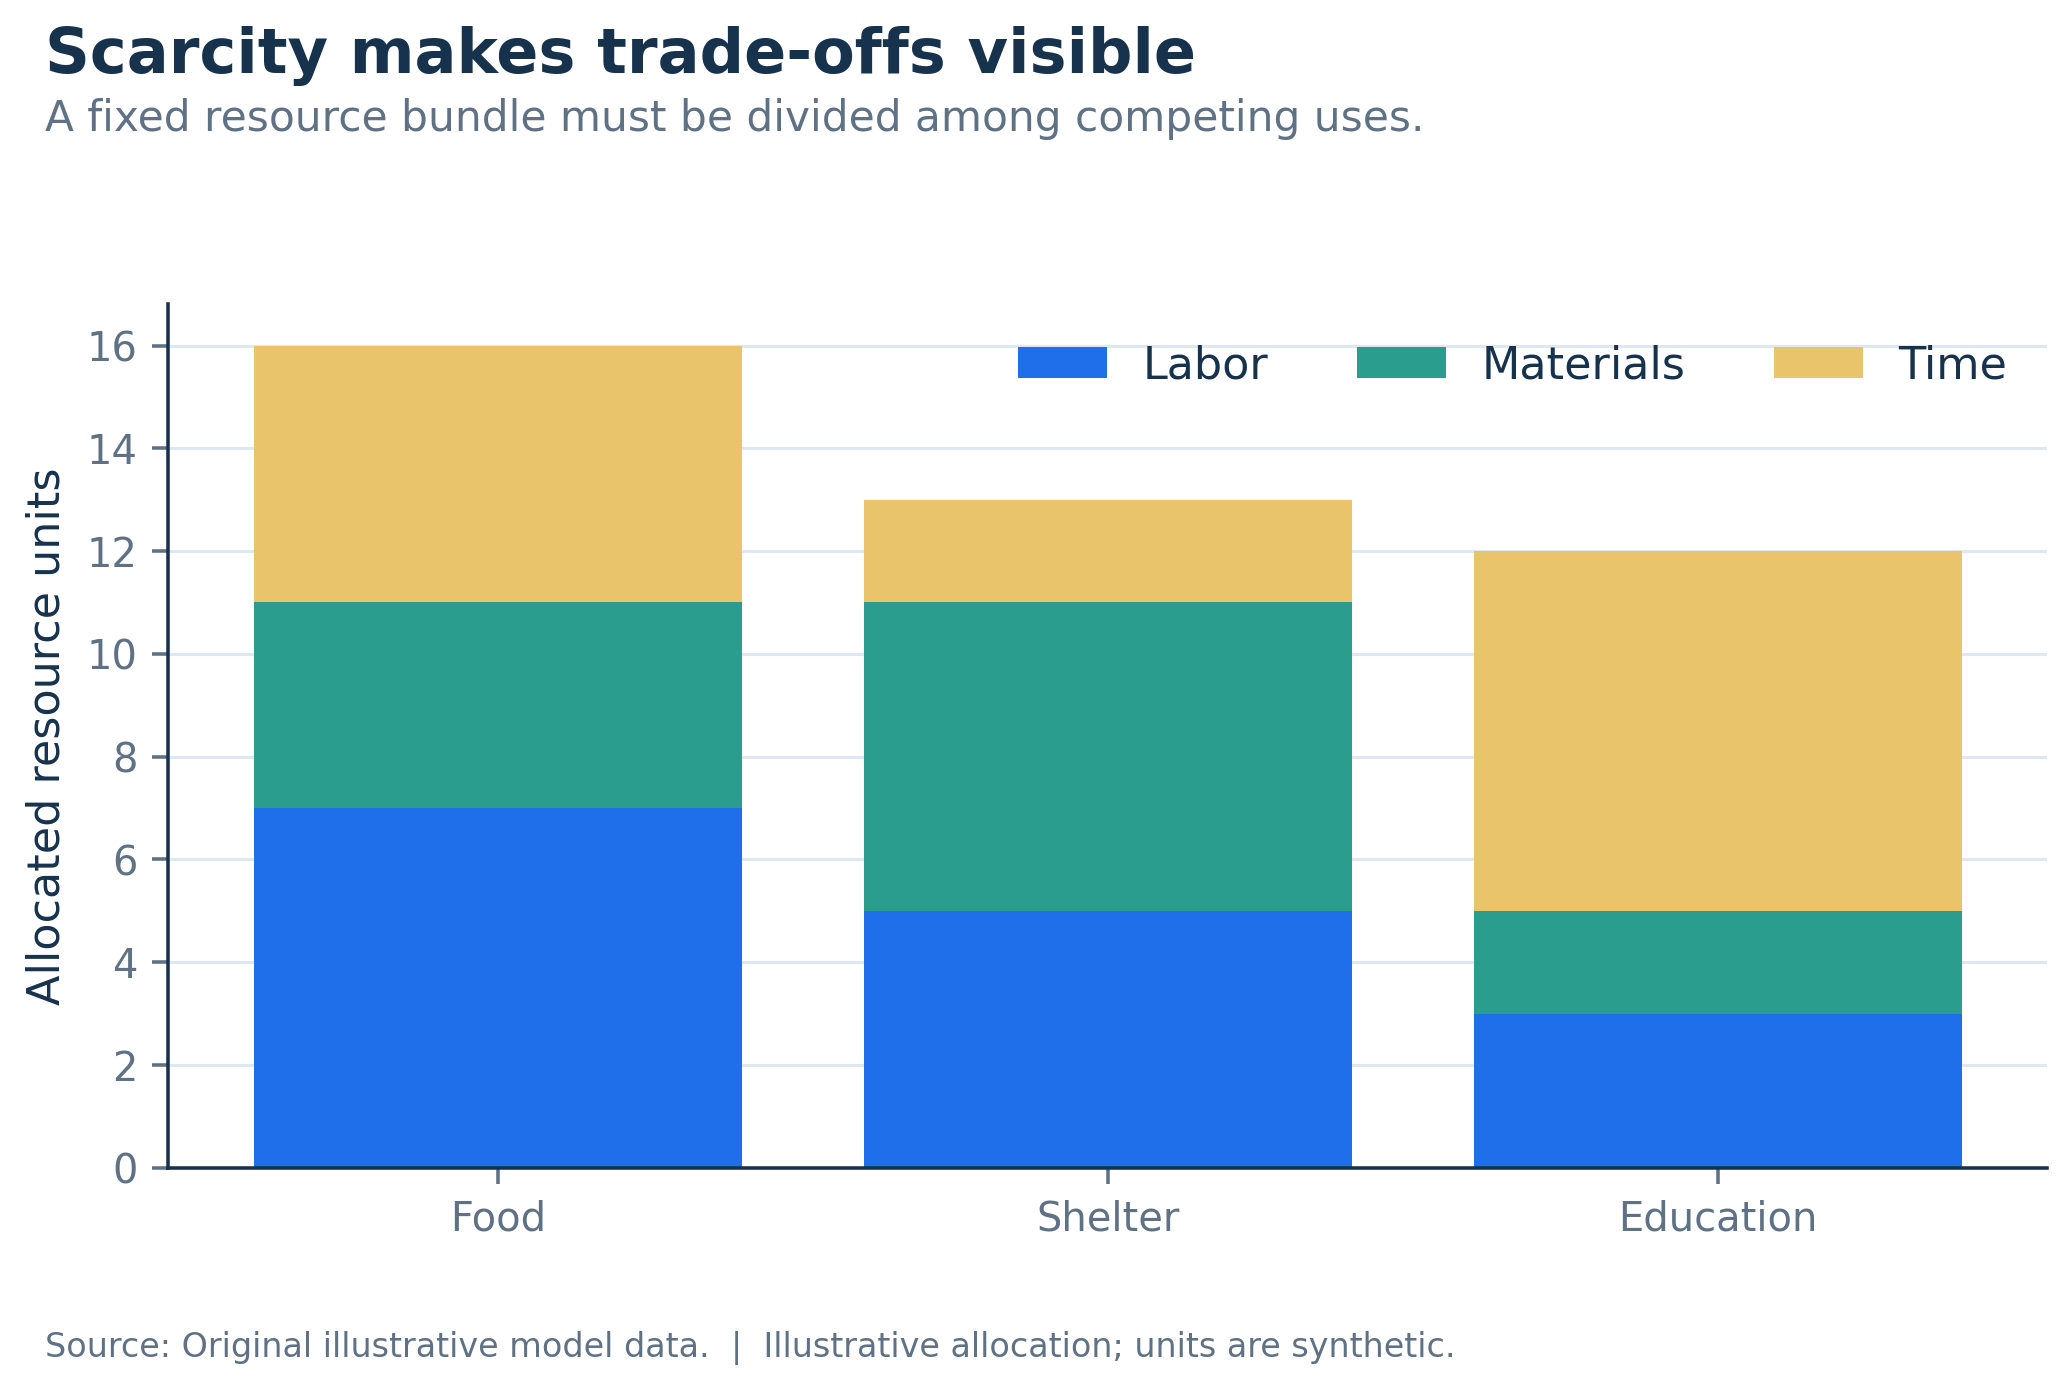
\includegraphics[width=0.90\linewidth,height=0.56\textheight,keepaspectratio]{session-01-three-resource-scarcity-panel.png}\column{0.35\textwidth}
    \only<1>{\vspace{0.8cm}\Large\blue{Read the bars.}\par\vspace{0.18cm}Which use receives the scarce bundle?}
    \only<2>{\vspace{0.25cm}\Large\blue{Name the constraints.}\par\vspace{0.15cm}\begin{itemize}\item labor\item materials\item time\end{itemize}}
    \only<3>{\vspace{0.25cm}\Large\orange{Trade-off}\par\vspace{0.18cm}More of one use requires less of another when the bundle is fixed.}
  \end{columns}
\end{frame}

% Choice: selection -> foregone alternative -> definition
\begin{frame}<1-3>{Opportunity cost names the benefit left behind}
  \begin{columns}[T,totalwidth=\textwidth]\column{0.56\textwidth}\centering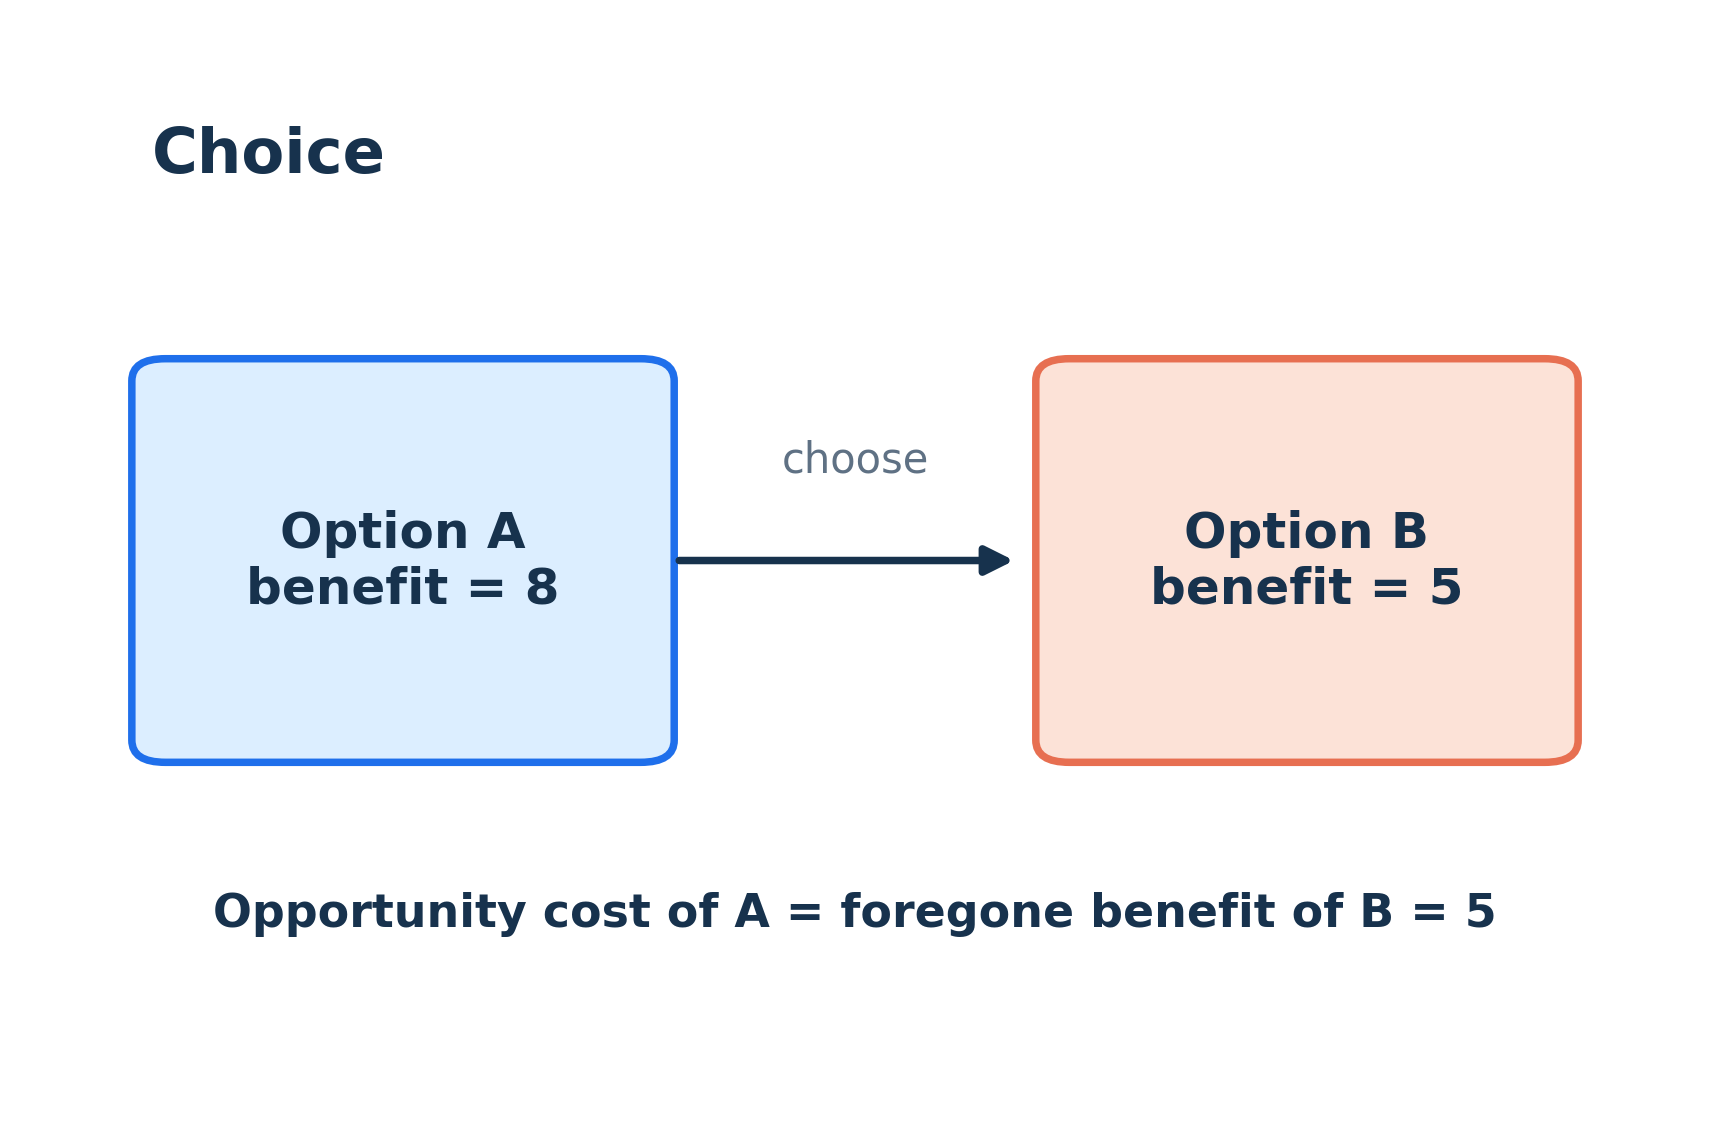
\includegraphics[width=0.82\linewidth,height=0.44\textheight,keepaspectratio]{session-01-choice-opportunity-cost-card.png}\column{0.37\textwidth}
    \only<1>{\vspace{0.55cm}\Large\blue{Choice}\par\vspace{0.18cm}The decision-maker chooses A.}
    \only<2>{\vspace{0.55cm}\Large\blue{What is given up?}\par\vspace{0.18cm}The next-best alternative is B.}
    \only<3>{\vspace{0.55cm}\Large\orange{Opportunity cost}\par\vspace{0.18cm}The benefit from B is the opportunity cost of choosing A.}
  \end{columns}
\end{frame}

% PPF bridge: curve -> points -> projections -> conclusion
\begin{frame}<1-4>{A movement along a boundary shows a trade-off}
  \begin{columns}[T,totalwidth=\textwidth]\column{0.64\textwidth}\centering
    \begin{tikzpicture}[x=0.50cm,y=0.29cm,>=Latex]
      \draw[->,thick,APBlue] (0,0) -- (11,0) node[below right,font=\sffamily\normalsize] {Good A};
      \draw[->,thick,APBlue] (0,0) -- (0,11) node[above left,font=\sffamily\normalsize] {Good B};
      \draw[very thick,APTeal] (0.5,9.5) .. controls (3.2,8.9) and (6.4,5.8) .. (9.8,0.7);
      \only<2->{\fill[APBlue] (3.2,7.9) circle (3pt) node[above right,font=\sffamily\normalsize] {A};\fill[APOrange] (6.6,4.7) circle (3pt) node[above right,font=\sffamily\normalsize] {B};}
      \only<3->{\draw[densely dashed,Muted] (3.2,0) -- (3.2,7.9) (0,7.9) -- (3.2,7.9);\draw[densely dashed,Muted] (6.6,0) -- (6.6,4.7) (0,4.7) -- (6.6,4.7);\draw[->,very thick,APOrange] (3.55,7.45) -- (6.15,5.15);}
    \end{tikzpicture}
  \column{0.30\textwidth}
    \only<1>{\vspace{0.7cm}\Large\blue{Start with the boundary.}\par\vspace{0.18cm}It shows feasible combinations of two goods.}
    \only<2>{\vspace{0.7cm}\Large\blue{Compare A and B.}\par\vspace{0.18cm}Both points lie on the same boundary.}
    \only<3>{\vspace{0.7cm}\Large\blue{Project to the axes.}\par\vspace{0.18cm}Good A rises while Good B falls.}
    \only<4>{\vspace{0.7cm}\Large\orange{Trade-off}\par\vspace{0.18cm}Moving from A to B gives up Good B.}
  \end{columns}
\end{frame}

% AP transfer: prompt -> evidence -> answer
\begin{frame}<1-3>{AP transfer: identify the scarce resource}
  \begin{columns}[T,totalwidth=\textwidth]\column{0.64\textwidth}\Large One empty classroom must serve either a tutoring center or a rehearsal room. Which statement is most accurate?\vspace{0.22cm}\begin{enumerate}\setlength{\itemsep}{0.10cm}\normalsize\item Scarcity exists only if the school charges rent.\item The room is scarce because it has alternative uses.\item There is no scarcity if both activities are valuable.\end{enumerate}\column{0.30\textwidth}
    \only<1>{\vspace{0.9cm}\muted{Read the choices first.}}
    \only<2>{\vspace{0.55cm}\Large\blue{Evidence}\par\vspace{0.18cm}The classroom is fixed and has alternative uses.}
    \only<3>{\vspace{0.35cm}\Large\orange{Answer: B}\par\vspace{0.18cm}The room cannot serve both uses at once.}
  \end{columns}
\end{frame}

% Exit ticket: prompt -> response -> model answer
\begin{frame}<1-3>{Exit ticket: state the causal chain}
  \only<1>{\vfill\prompt{Because \underline{\hspace{1.5cm}} is limited, choosing \underline{\hspace{1.5cm}} means giving up \underline{\hspace{1.5cm}}.}\vfill}
  \only<2>{\vspace{0.6cm}\begin{block}{Write one accurate causal sentence}\large Because \answerline\ is limited, choosing \answerline\ means giving up \answerline.\end{block}\vfill\begin{center}\muted{Use one scarce resource, one choice, and one foregone alternative.}\end{center}}
  \only<3>{\vspace{0.6cm}\begin{block}{Model answer}\large Because \blue{classroom space} is limited, choosing \blue{a tutoring center} means giving up \orange{a rehearsal room}.\end{block}\vfill\begin{center}\Large\blue{scarce resource} $\longrightarrow$ \blue{choice} $\longrightarrow$ \orange{trade-off}\end{center}}
\end{frame}

\end{document}
